% ---- start of strainratemeaning.tex -----------------------------------
\section{Meaning of terms in strain rate tensor}
\label{strainratemeaning}

Figure \ref{fluidelement} shows how a fluid element deforms during its motion. The deformation can be analysed into different modes and the respective strains and strain rates can be expressed in terms of the velocity gradients as shown below.


\begin{figure}[h]
\framebox{
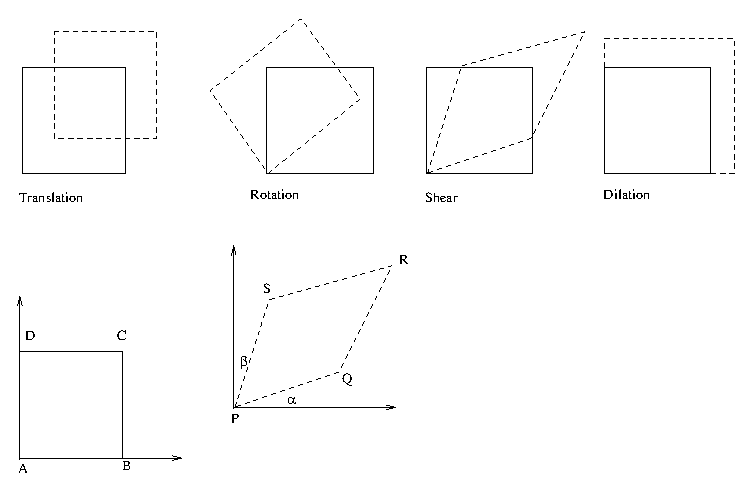
\includegraphics{images/a13-strainrate.eps}
}
\caption{Analysis of deformation of a fluid element}
\label{fluidelement}
\end{figure}

\setlength{\parskip}{5mm}
\setlength{\parindent}{0mm}


In this handout, the geometry is restricted to 2D and the symbols used are $x,y$ for axes, $u,v$ for velocity components along those axes, respectively, for easy observation. The results can be extended to 3D using subscript notation.


Initial Positions:

\begin{tabular}{|l|l|l|}
\hline
$A$ & $x_0$ & $y_0$ \\

$B$ & $(x_0 + \Delta x)$ & $y_0$ \\

$C$ & $(x_0 + \Delta x)$ & $(y_0 + \Delta y)$ \\

$D$ & $x_0$ & $(y_0 + \Delta y)$ \\
\hline
\end{tabular}

Velocities:

\begin{tabular}{|l|l|l|}
\hline

$A$ & $u$ & $v$ \\

$B$ & $(u + \frac{\partial u}{\partial x} \Delta x)$ & $(v + \frac{\partial v}{\partial x} \Delta x)$ \\

$C$ & $(u + \frac{\partial u}{\partial x} \Delta x + \frac{\partial u}{\partial y} \Delta y)$ & $(v + \frac{\partial v}{\partial x} \Delta x + \frac{\partial v}{\partial y} \Delta y))$ \\

$D$ & $(u + \frac{\partial u}{\partial y} \Delta y)$ & $(v + \frac{\partial v}{\partial y} \Delta y)$ \\
\hline
\end{tabular}


Positions after $dt$:

\begin{tabular}{|l|l|l|}
\hline

$P$ & $x_0 + u dt$ & $y_0 + v dt$ \\

$Q$ & $(x_0 + \Delta x) + (u + \frac{\partial u}{\partial x}\Delta x) dt$ & 
$y_0 + (v + \frac{\partial v}{\partial x}\Delta x) dt$ \\

$R$ & $(x_0 + \Delta x) + (u + \frac{\partial u}{\partial x}\Delta x + \frac{\partial u}{\partial y}\Delta y) dt$ & 
$(y_0 + \Delta y)+ (v + \frac{\partial v}{\partial x}\Delta x + \frac{\partial v}{\partial y}\Delta y) dt$ \\


$S$ & $x_0 + (u + \frac{\partial u}{\partial y}\Delta y) dt$ & 
$(y_0 + \Delta y) + (v + \frac{\partial v}{\partial y}\Delta y) dt$  \\

\hline

\end{tabular}


Dilational strain along $x$, $s_{11}$ is $\frac{PQ_x-AB}{AB}$. 
Shear strain along $y$, $s_{12}$ is $\frac{PQ_y}{AB}$. 

Dilational strain along $y$, $s_{22}$ is $\frac{PS_y-AD}{AD}$. 
Shear strain along $x$, $s_{21}$ is $\frac{PS_x}{AD}$. 

Dilational Strain rate:
$$ e_{11} = \frac{\frac{\partial u}{\partial x} \Delta x dt}{\Delta x} \frac{1}{dt} = \frac{\partial u}{\partial x} $$
$$ e_{22} = \frac{\frac{\partial v}{\partial y} \Delta y dt}{\Delta y} \frac{1}{dt} = \frac{\partial v}{\partial y} $$

Shear Strains:
$$\alpha = \frac{\frac{\partial v}{\partial x} \Delta x dt}{\Delta x} = \frac{\partial v}{\partial x} dt$$
$$\beta = \frac{\frac{\partial u}{\partial y} \Delta y dt}{\Delta y} = \frac{\partial u}{\partial y} dt$$
Pure shear strain rate:
$$e_{12} = e_{21} = \frac{1}{2} (\alpha + \beta) \frac{1}{dt} = \frac{1}{2} \left( \frac{\partial v}{\partial x} + \frac{\partial u}{\partial y} \right) $$
Pure rotational rate:
$$\Omega_{12} = -\Omega_{21} = \frac{1}{2} (\alpha - \beta) \frac{1}{dt} = \frac{1}{2} \left( \frac{\partial v}{\partial x} - \frac{\partial u}{\partial y} \right) $$

One can say generalize the above expressions using the subscript notation in the following way:

General strain rate tensor: $$ s_{ij} = {\partial u_i \over \partial x_j}$$

Expressing it as a sum of symmetric ($e_{ij}$) and anti-symmetric $(\Omega_{ij})$ tensors:
$$ s_{ij} = e_{ij} + \Omega_{ij}$$
	
Dilation: $$s_{ij} \delta_{ij} = s_{ii} = e_{ii} = {\partial u_i \over \partial x_i}$$ 
Shear: $${1 \over 2} \left( s_{ij} + s_{ji} \right) = {\partial u_i \over \partial x_j} + {\partial u_j \over \partial x_i}$$
Rotation: $${1 \over 2} \left( s_{ij} - s_{ji} \right) = {\partial u_i \over \partial x_j} - {\partial u_j \over \partial x_i}$$

% ------- end of strainratemeaning.tex ------------------
